\documentclass[../thesis.tex]{subfiles}

\begin{document}

\chapter{The Daya Bay experiment}
\label{chap:experim}

\section*{Introduction}

The Daya Bay experiment was designed to measure $\theta_{13}$ by observing the antineutrinos produced by the six 2.9~GWth nuclear reactors of the Daya Bay and Ling Ao power plants, located near Shenzhen in southern China. A total of eight functionally identical antineutrino detectors (ADs) were deployed, each containing a target of 20~tons of gadolinium-doped liquid scintillator (GdLS). Four of the ADs were evenly divided among two near halls ($\sim$350-600~m baselines from the cores), and the remaining four were placed in a single far hall ($\sim$1500-1950~m baselines). Shielding from cosmic rays was provided by $\sim$100~m and $\sim$300~m, respectively, of mountainous overburden at the near and far halls. The ADs in each hall were immersed in instrumented water pools which provided shielding from ambient radioactivity and detection of Cerenkov radiation from atmospheric muons. Redundant detection of muons, as well as directional information, were made available by resistive plate chambers (RPCs) laid on top of the water pools. This chapter provides a detailed account of the layout, detectors, and shielding/vetoing system of the experiment.

\section{Site layout}
\label{sec:expLayout}

\begin{figure}[ht]
  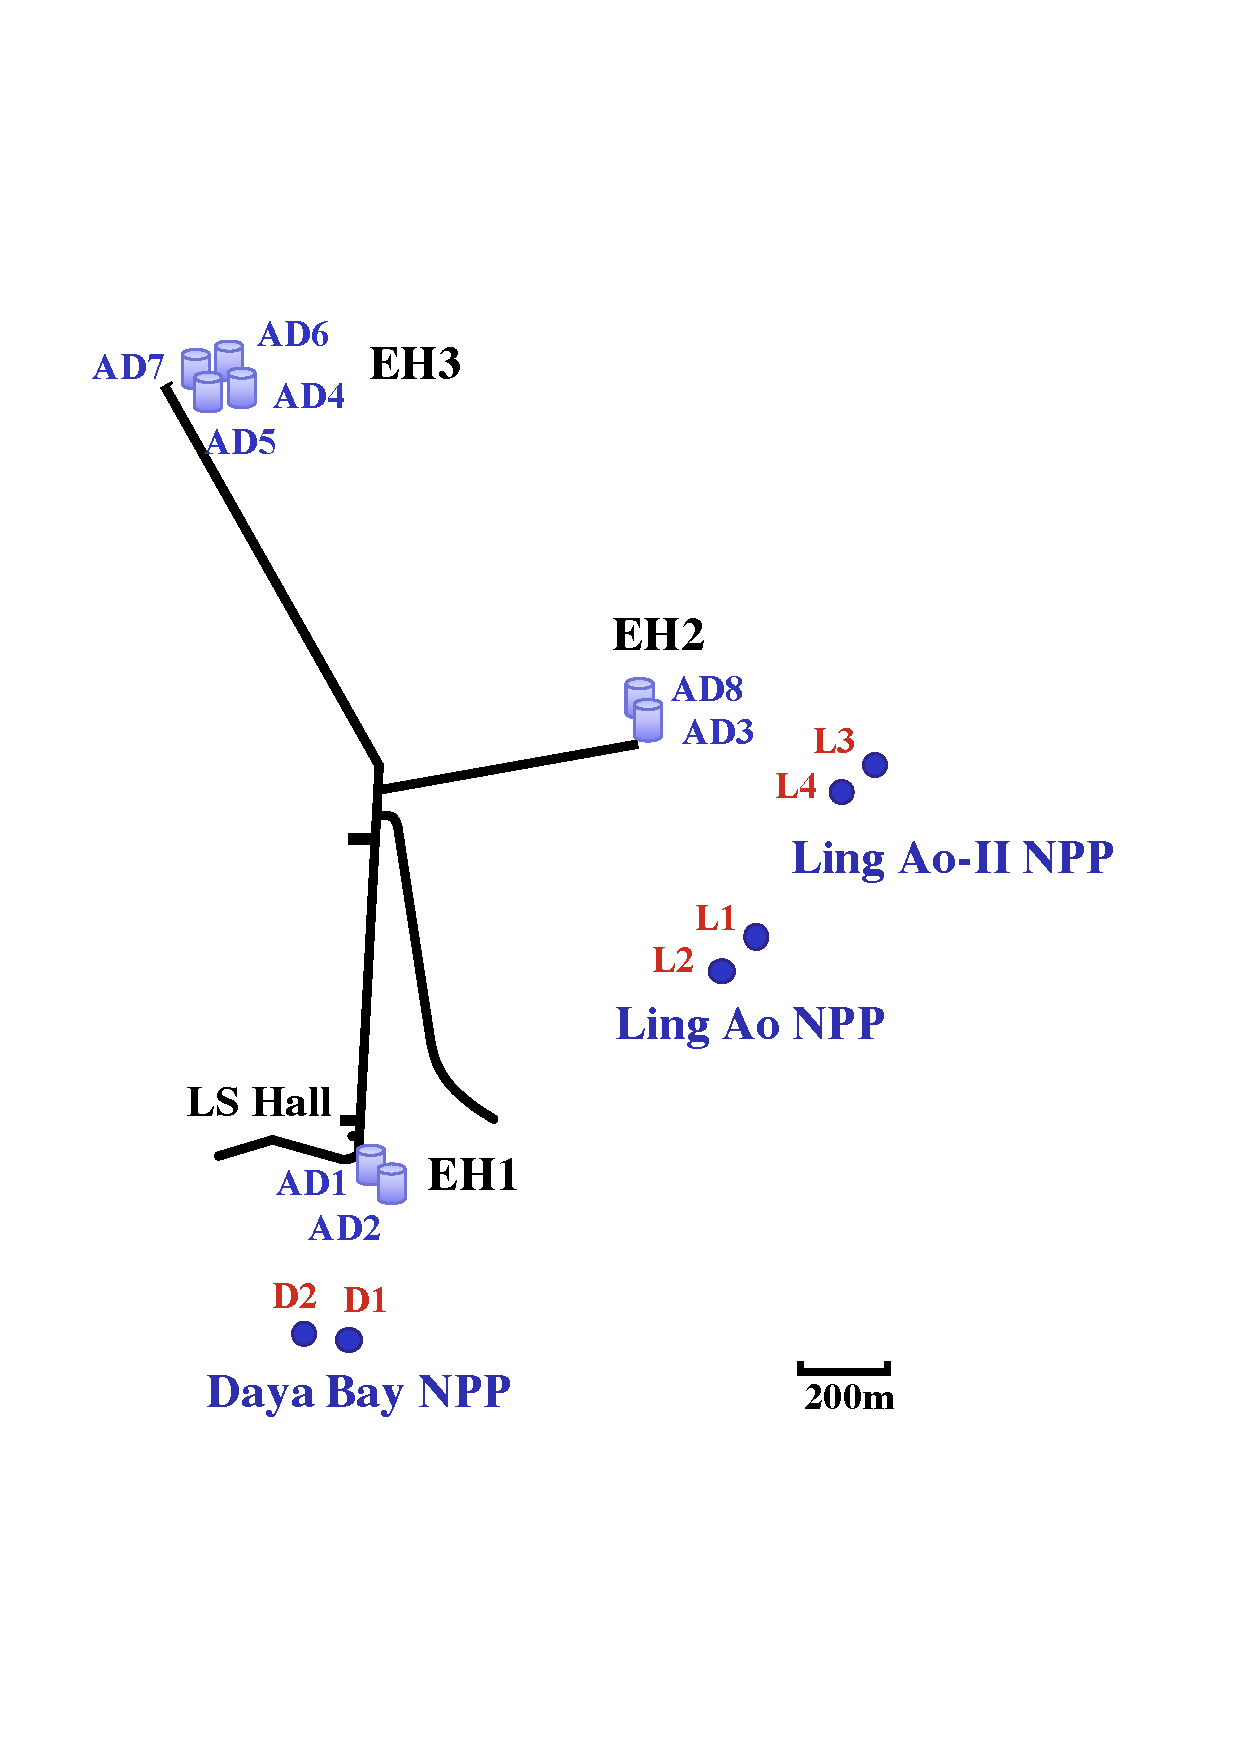
\includegraphics[scale=0.4]{layout.pdf}
  \caption{The layout of the Daya Bay experiment.}
  \label{fig:layout} 
\end{figure}

As shown in \autoref{fig:layout}.

\section{Antineutrino detectors}
\label{sec:expADs}

\begin{figure}[ht]
  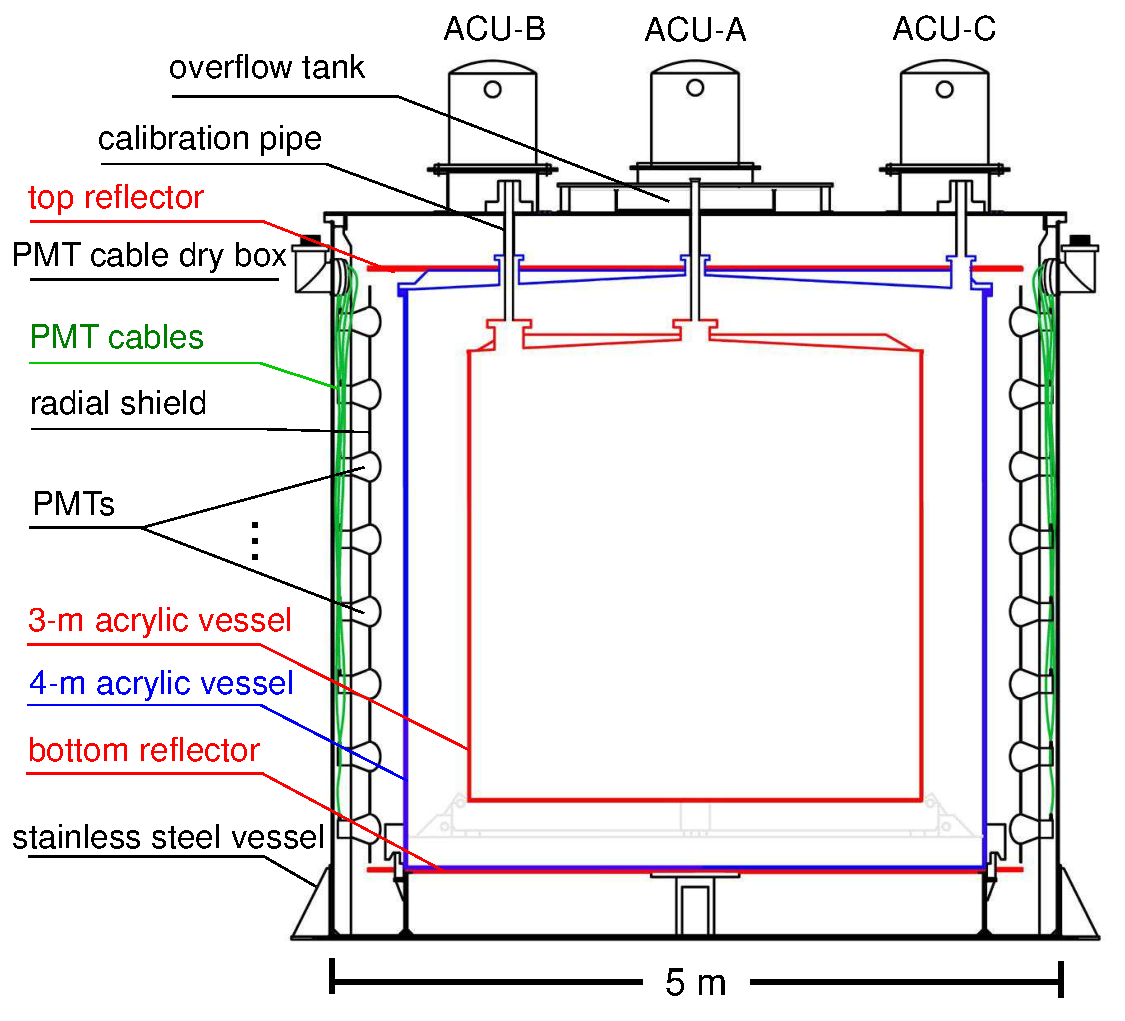
\includegraphics[scale=0.4]{exp_AD_structure.pdf}
  \caption{Structure of a Daya Bay antineutrino detector. From \cite{An_2017}.}
  \label{fig:expDetector}
\end{figure}


\subsection{Detection principle}
\label{sec:expDetPrinc}

\begin{figure}[ht]
  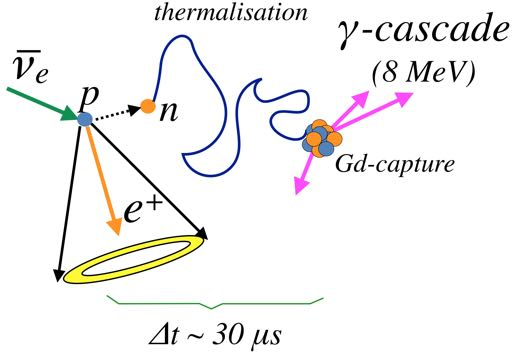
\includegraphics[scale=0.4]{ibd.png}
  \caption{The inverse beta decay reaction. Unlike a water Cerenkov detector, a Daya Bay AD cannot discern the direction of the positron. From \cite{Fernandez_2017}.}
  \label{fig:expIBD}
\end{figure}

\autoref{sec:baryonAsym} discusses the baryon asymmetry while \autoref{sec:expADs} describe the detectors.

\section{Shielding/vetoing system}
\label{sec:expShieldVeto}

\begin{figure}[ht]
  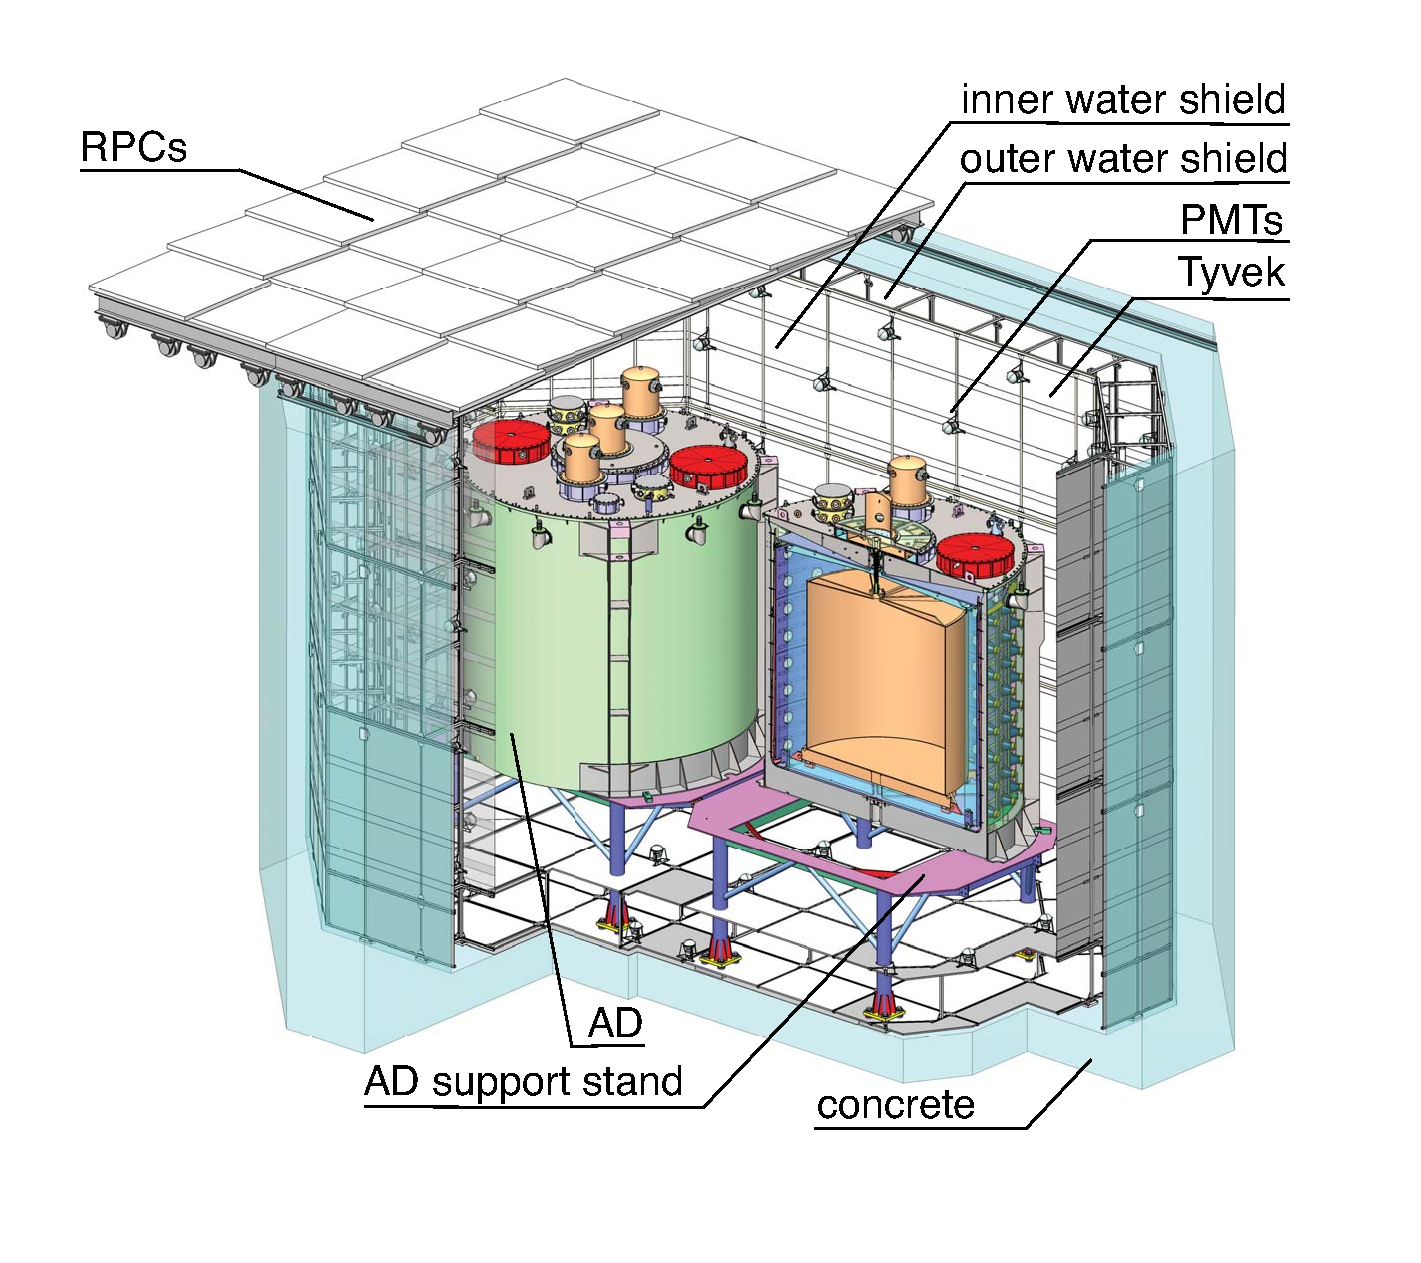
\includegraphics[scale=0.4]{exp_near_site_diagram.pdf}
  \caption{Water pool (including ADs) as configured in the near halls. The far hall is similar, with four ADs instead of two. From \cite{An_2017}.}
  \label{fig:expPool}
\end{figure}

\subfilebackmatter

\end{document}